\documentclass[10pt,A4]{article}
\usepackage[top=0.85in,left=2.75in,footskip=0.75in]{geometry}

% Use adjustwidth environment to exceed column width (see example table in text)
\usepackage{changepage}

% Use Unicode characters when possible
\usepackage[utf8]{inputenc}
\usepackage{booktabs,caption,fixltx2e}
\usepackage[flushleft]{threeparttable}
\usepackage{tabularx}
% textcomp package and marvosym package for additional characters
\usepackage{textcomp,marvosym}

% fixltx2e package for \textsubscript
\usepackage{fixltx2e}

% amsmath and amssymb packages, useful for mathematical formulas and symbols
\usepackage{amsmath,amssymb}

% cite package, to clean up citations in the main text. Do not remove.
\usepackage{cite}

% Use nameref to cite supporting information files (see Supporting Information section for more info)
\usepackage{nameref,hyperref}

% line numbers
\usepackage[right]{lineno}

% ligatures disabled
\usepackage{microtype}
%\DisableLigatures[f]{encoding = *, family = * }

% rotating package for sideways tables
\usepackage{rotating}

% Remove comment for double spacing
\usepackage{setspace} 
\doublespacing

% Text layout
\raggedright
\setlength{\parindent}{0.5cm}
\textwidth 5.25in 
\textheight 8.75in

% Bold the 'Figure #' in the caption and separate it from the title/caption with a period
% Captions will be left justified
\usepackage[aboveskip=1pt,labelfont=bf,labelsep=period,justification=raggedright,singlelinecheck=off]{caption}

% Use the PLoS provided BiBTeX style
\bibliographystyle{plos2015}

% Remove brackets from numbering in List of References
\makeatletter
\renewcommand{\@biblabel}[1]{\quad#1.}
\makeatother

% Leave date blank
\date{}

% Header and Footer with logo
\usepackage{lastpage,fancyhdr,graphicx}
\usepackage{ragged2e}

\usepackage{color}
\usepackage[dvipsnames]{xcolor}

%\usepackage{epstopdf}
\pagestyle{myheadings}
\pagestyle{fancy}
\fancyhf{}
\lhead{
%
\includegraphics[width=1.6in]{figures/pone.png}
}
\rhead{Calibration of a Density-based Model of Urban Morphogenesis\vspace{2mm}}
\rfoot{\thepage}
\renewcommand{\footrule}{\hrule height 2pt \vspace{2mm}}
\fancyheadoffset[L]{2.25in}
\fancyfootoffset[L]{2.25in}
%\lfoot{\sf Raimbault, 2017}
\lfoot{}

%% Include all macros below

\newcommand{\lorem}{{\bf LOREM}}
\newcommand{\ipsum}{{\bf IPSUM}}

%%%%%%%%%%%%%%%%%%%%%%
%% User-defined commands
%%%%%%%%%%%%%%%%%%%%%%


%Yoann's commands
\newcommand{\reels}{\mathbb{R}}
\newcommand{\naturels}{\mathbb{N}}
\newcommand{\relatifs}{\mathbb{Z}}
\newcommand{\rat}{\mathbb{Q}}
\newcommand{\complex}{\mathbb{C}}
\newcommand{\esp}{\mathbb{E}}
\newcommand{\proba}{\mathbb{P}}
\newcommand{\var}{\operatorname{Var}}
\newcommand{\cov}{\operatorname{Cov}}
\newcommand{\Tau}{\mathrm{T}}



% writing utilities

% comments and responses
\usepackage{xparse}
\DeclareDocumentCommand{\comment}{m o o o o}
{%
    \textcolor{red}{#1}
    \IfValueT{#2}{\textcolor{blue}{#2}}
    \IfValueT{#3}{\textcolor{ForestGreen}{#3}}
    \IfValueT{#4}{\textcolor{red!50!blue}{#4}}
    \IfValueT{#5}{\textcolor{Aquamarine}{#5}}
}


% todo
\newcommand{\todo}[1]{\textcolor{red!50!blue}{\textbf{\textit{#1}}}}




%% END MACROS SECTION


\begin{document}
\vspace*{0.35in}


\justify









%\end{document}





\section*{S3 Text : Sensitivity of indicators to spatial resolution}

We evaluate here the sensitivity of morphological indicators to grid size. We show in Fig.~\ref{fig:app:staticcorrelations:sensitivity-maps-morpho} morphological indicators, mapped for France, for different grid sizes. The sizes taken here, in correspondance to the 50km scale used in main results, are at similar magnitudes: we test windows of size 30km and 100km. The offsets are in each case half of the window (15km and 50km respectively). It is possible to see with eyeball validation that some indicators have a low sensitivity, the change in scale resembling a smoothing of the finer field: for example for morphology in the case of Moran, entropy and hierarchy. Average distance, which is indeed rather noisy at the smaller scale, is necessarily sensitive to aggregation, what is consistent with a sensitivity expected at smoothing. 


%%%%%%%%%%%%
\begin{figure}
	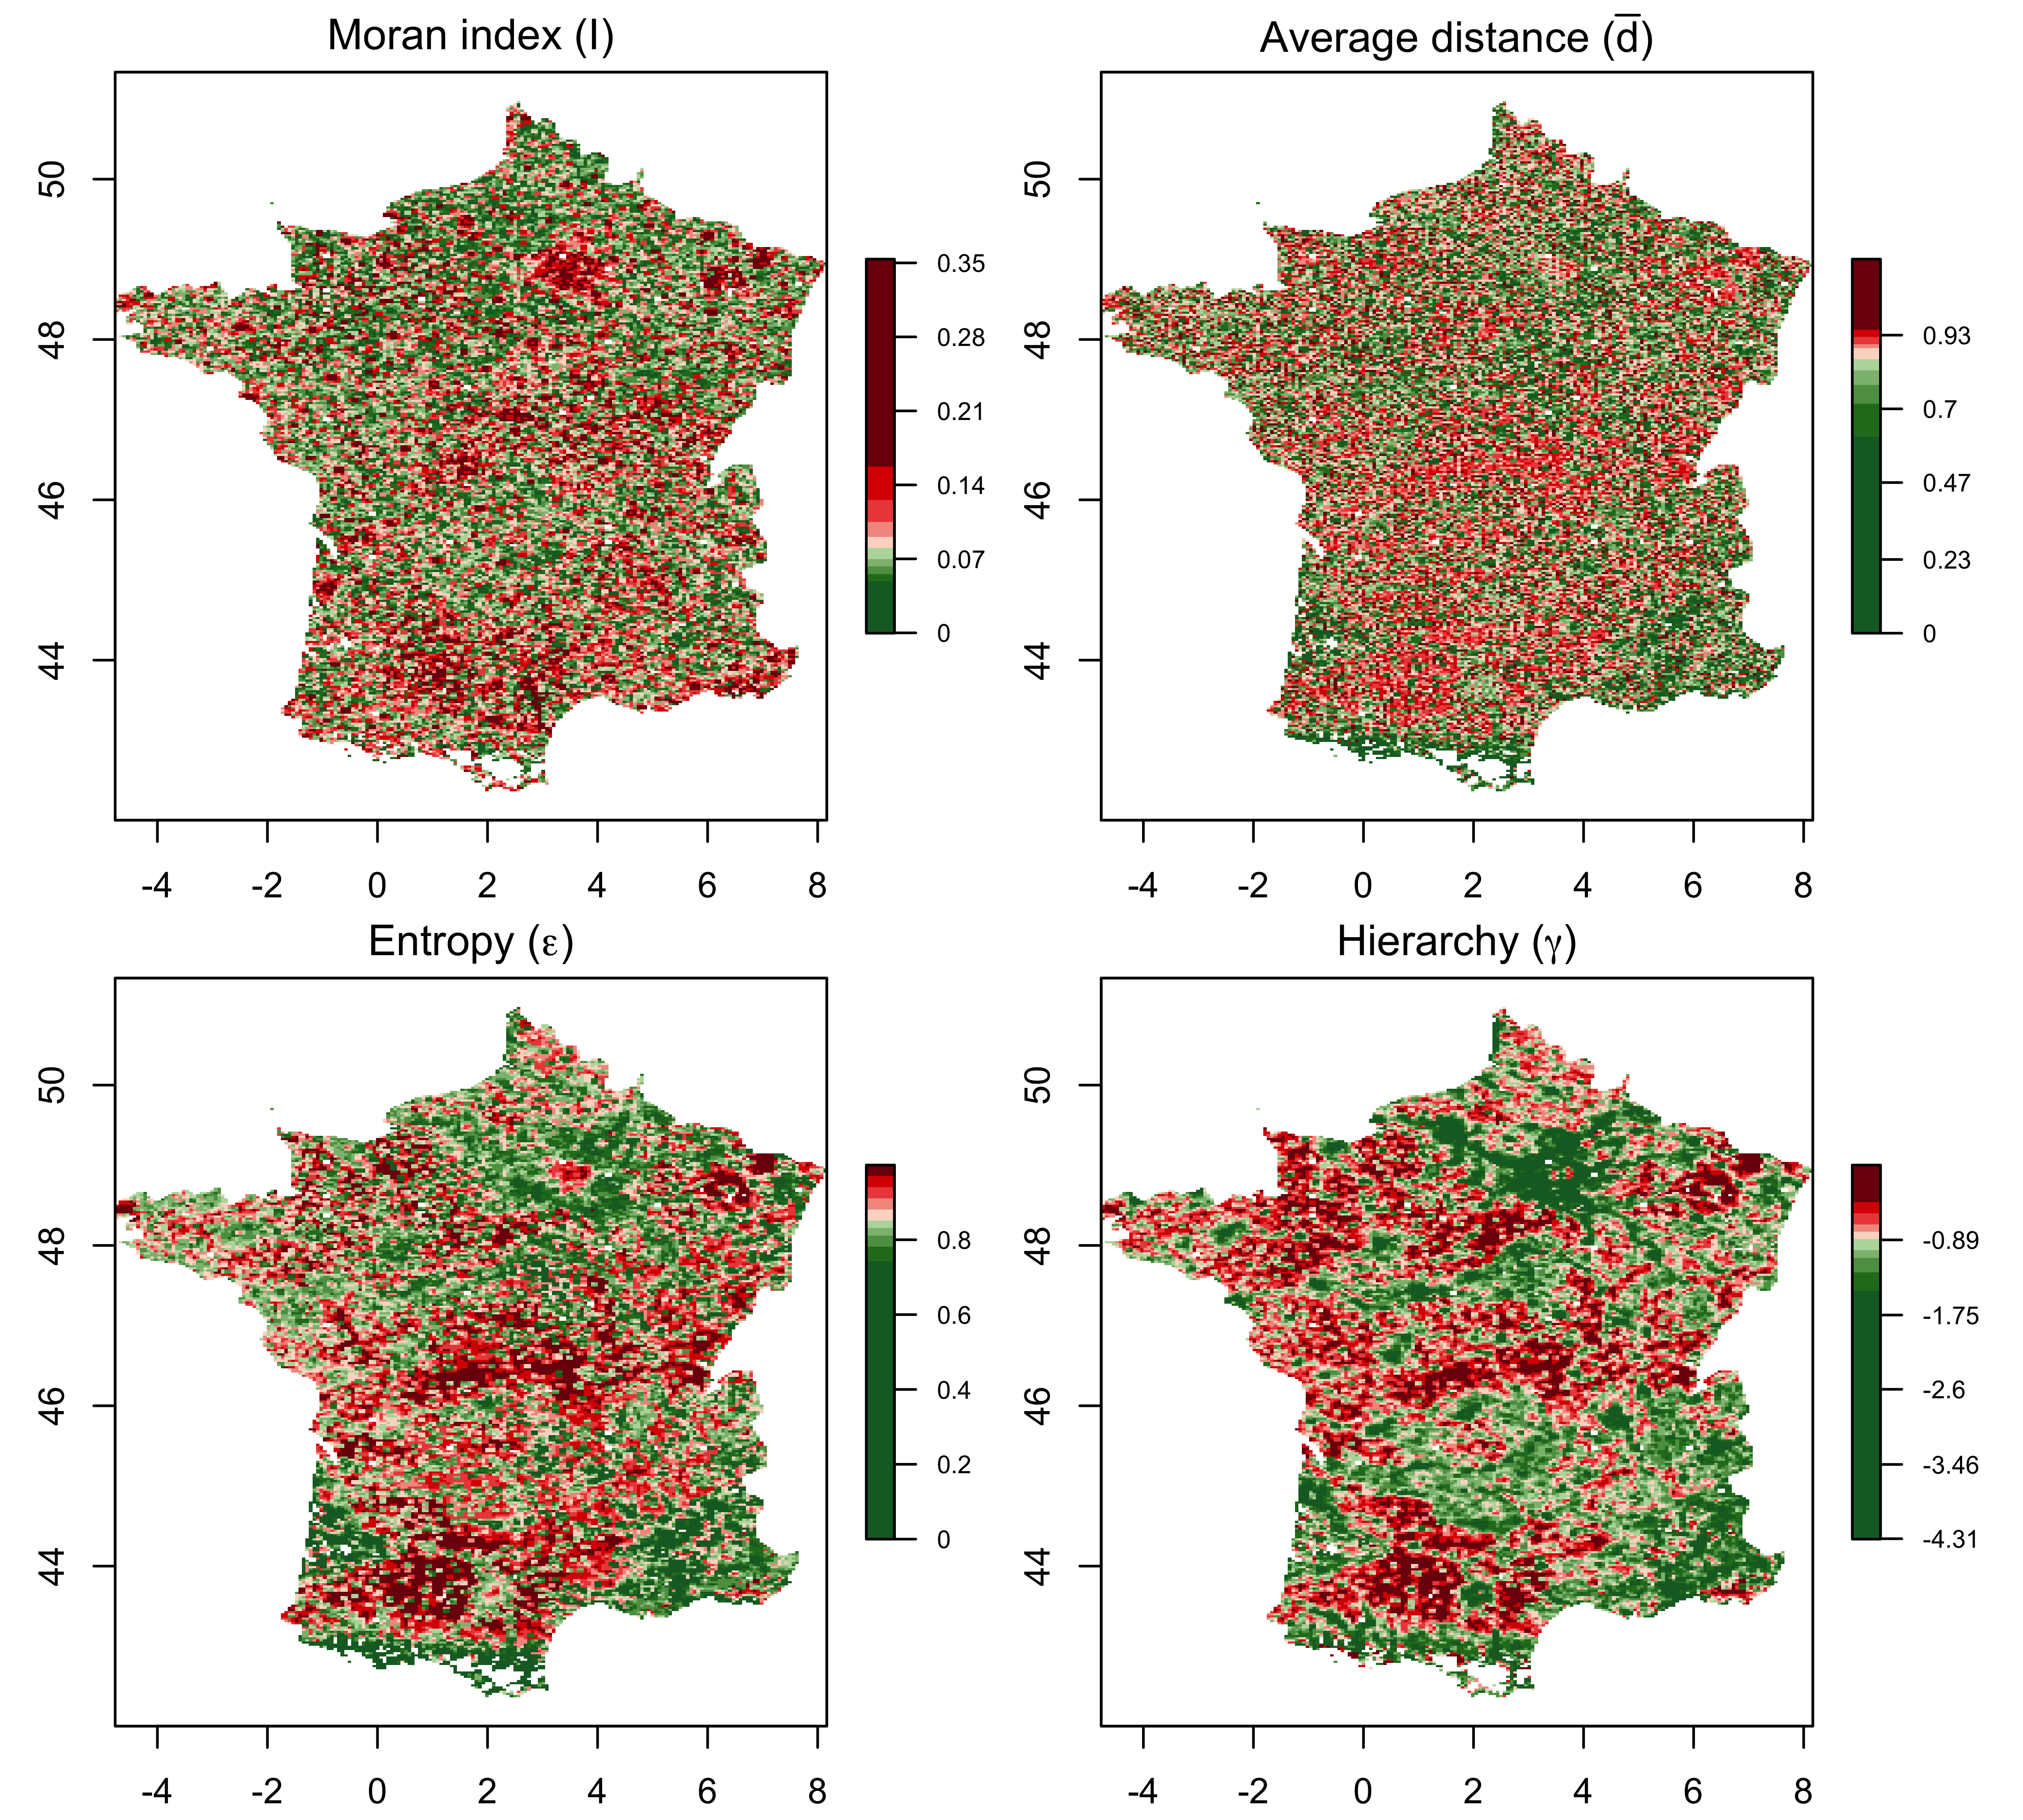
\includegraphics[width=\linewidth,height=0.48\textheight]{figuresraw/indics_morpho_en_areasize60_offset30_factor0_5.png}\\
	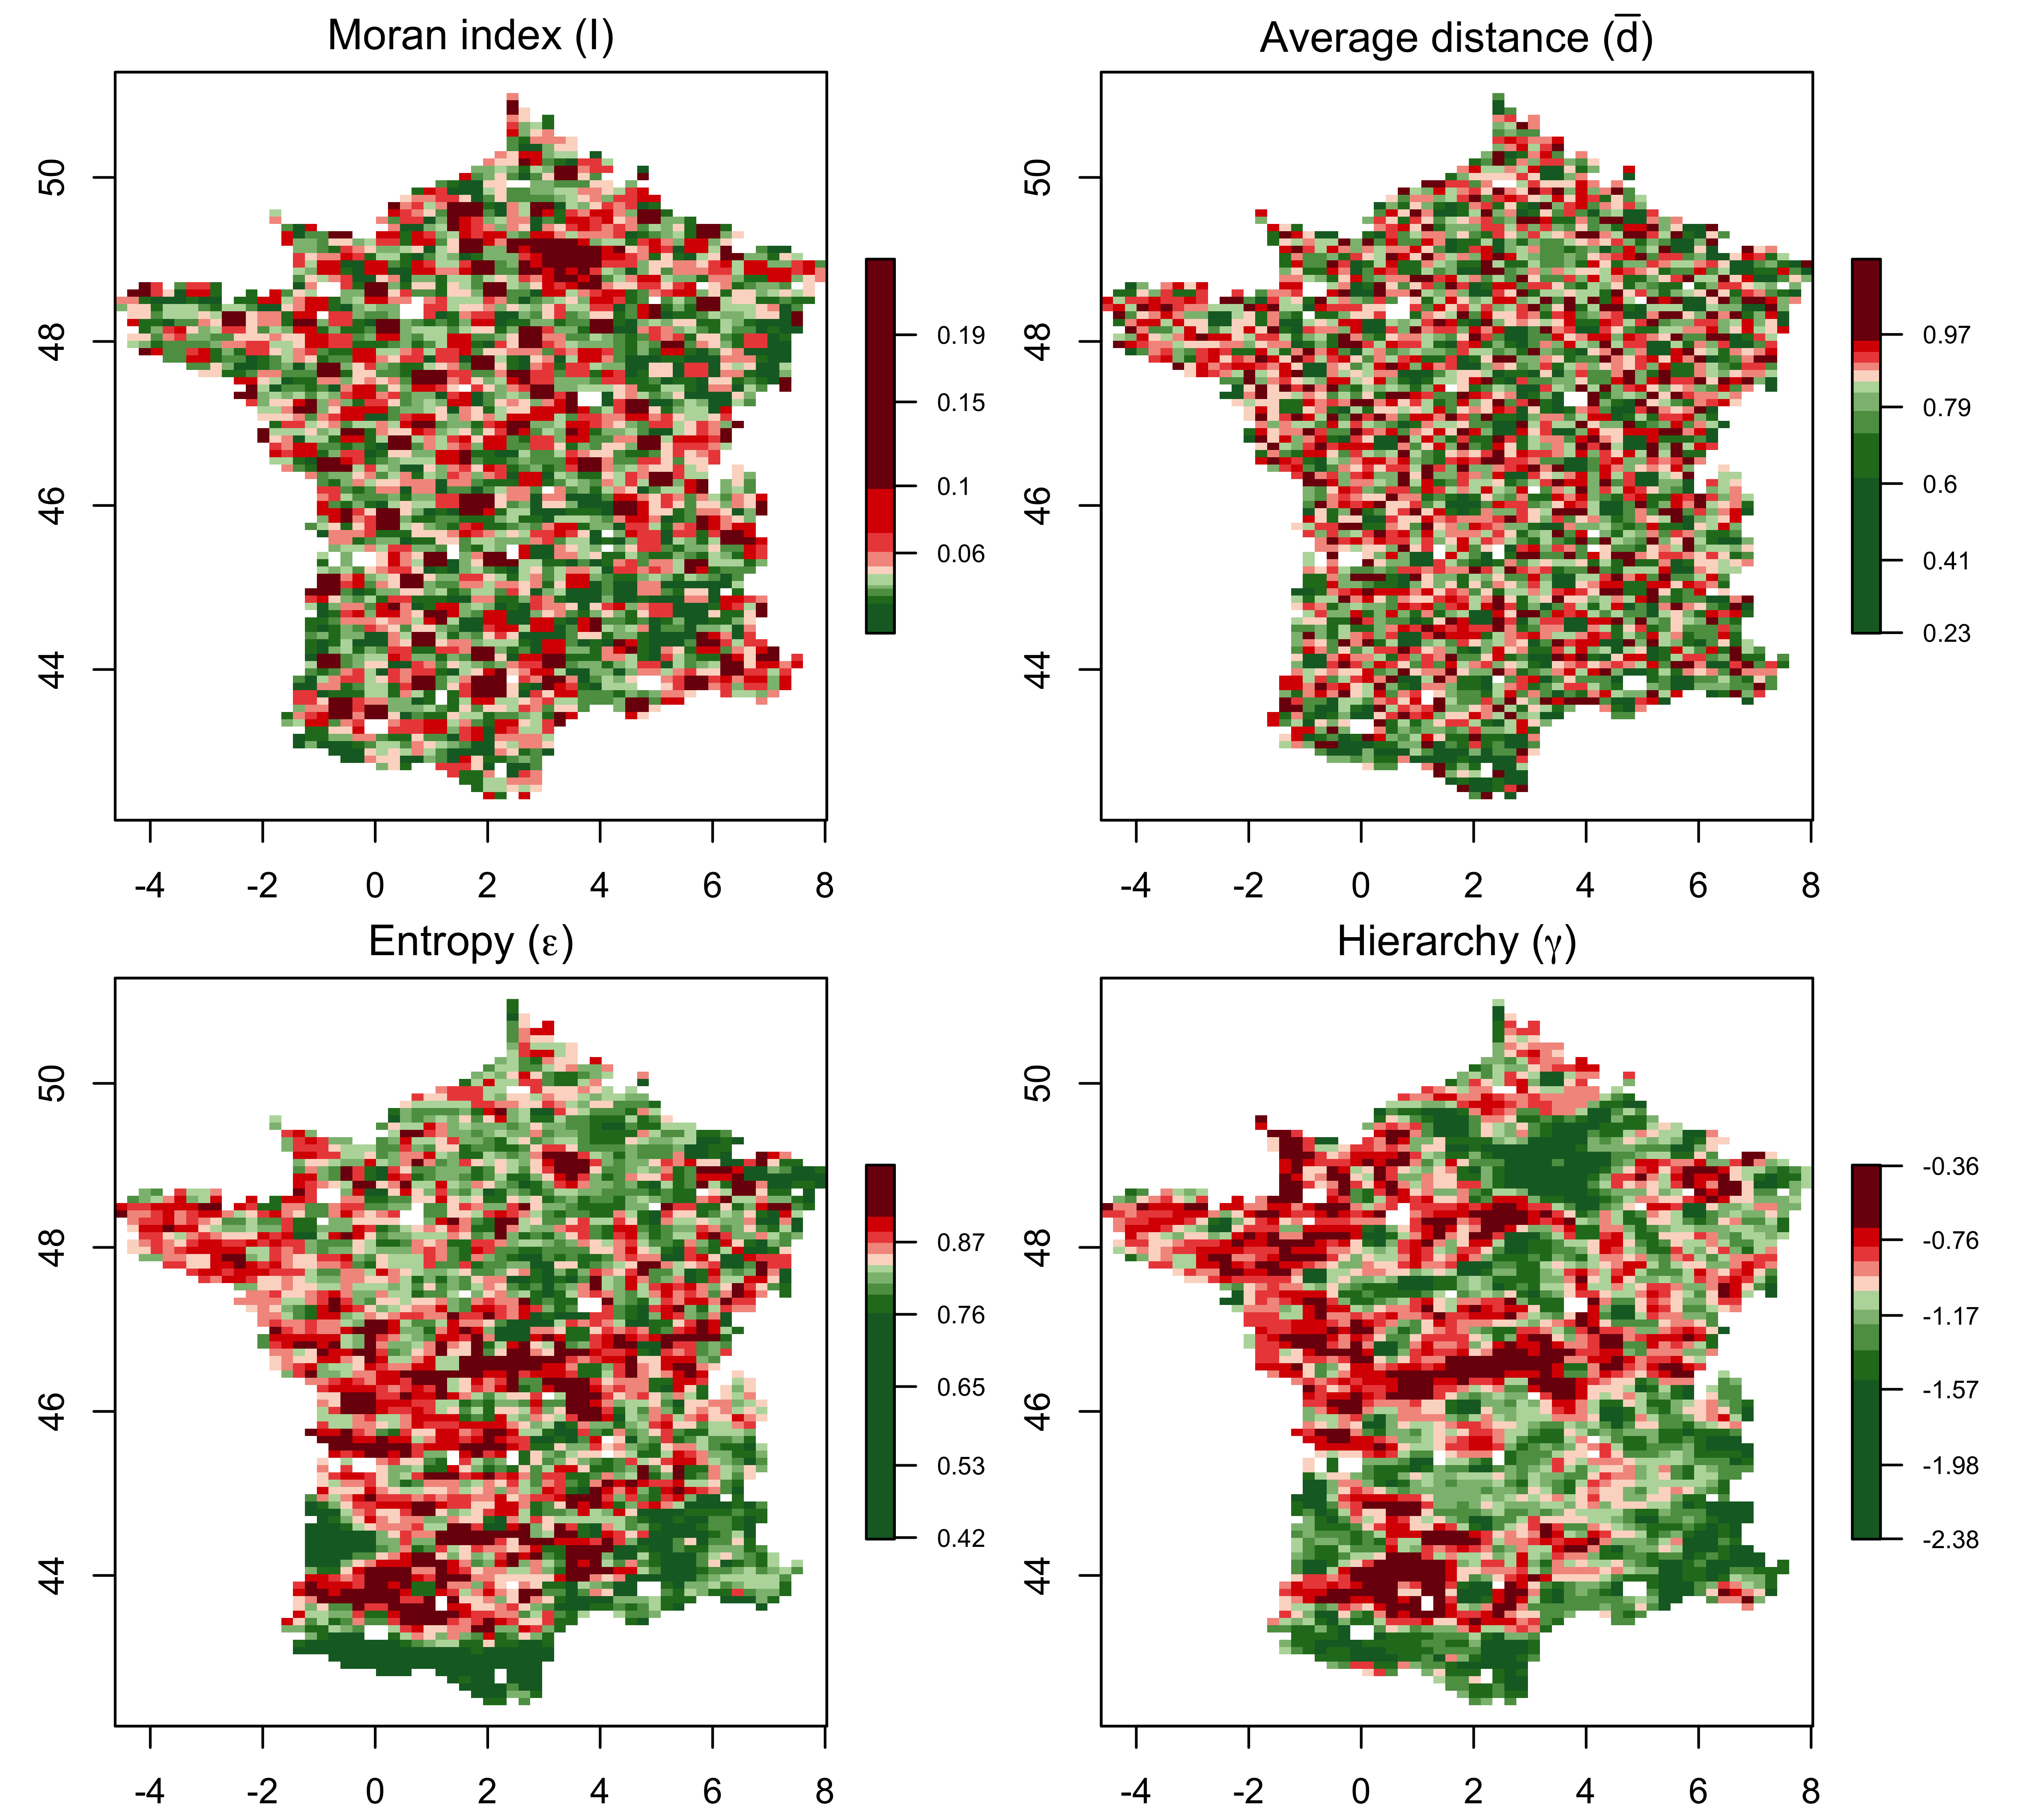
\includegraphics[width=\linewidth,height=0.48\textheight]{figuresraw/indics_morpho_en_areasize200_offset100_factor0_5.png}
	\caption{\textbf{Morphological indicators for different grid sizes.} The first four maps show the indicators computed on a window of size 30km, the last four maps with a window of size 100km.\label{fig:app:staticcorrelations:sensitivity-maps-morpho}}
\end{figure}
%%%%%%%%%%%%


This comparison, on the one hand is to be taken with caution because of the difficulty to directly compare scales for indicators, and on the other hand stays limited. We propose then a method to quantify the variability of indicators to window size. Let $X_D$ and $X_d$ two spatial fields corresponding to two spatial scales $D > d$ (that we take as characteristic distances). The fields are assumed discrete at points respectively denoted by $\left(\vec{x}_i^{(D)}\right)_{1 \leq i \leq N_D}$ and $\left(\vec{x}_j^{(d)}\right)_{1 \leq i \leq N_d}$. The idea is to compare a smoothing of the finer field to the field with the larger scale: if the correlation between these two values is high, it is possible to deduce one field from the other by aggregation and the scale of computation does not influence final results in an other way than the final resolution. Let $W_{ij} = \left( \exp{ - d_{ij} / d_0} \right)_{ij}$ a matrix of spatial weights computed with euclidian distances $d_{ij}$ between the points $\vec{x}_i^{(D)}$ and $\vec{x}_j^{(d)}$. Then with $W'_{ij} = W_{ij} / \sum_j W_{ij}$, we can compute the spatial smoothing of $X_d$ at the points $\vec{x}_i^{(D)}$, with the matrix product
\[
\tilde{X}_d (\vec{x}_i^{(D)}) = W' \ast \vec{x}_j^{(d)}
\]
The correlation is then given by $\rho\left[\tilde{X}_d,X_D\right]$ estimated on all $\vec{x}_i^{(D)}$ points.



The Fig.~\ref{fig:app:staticcorrelations:sensitivity-corrs} gives the variation of this correlation for all $(D,d)$ couples, with a variable $d_0$ for smoothing. We generally observe the existence of a maximum, which corresponds to the optimal smoothing level to deduce the larger scale from the finer. The largest correlations on all indicators are obtained for $D=50$km and $d=30$km, what means that indicators are not very sensitive to small variations in small window sizes. As expected, the lowest correlations are obtained for the largest scale difference (100/30km). Morphological indicators have the same qualitative behavior across combinations, and we find the behavior suggested by the previous maps (entropy and hierarchy being the less sensitive, Moran index and average distance a bit more sensitive). For all indicators, the sensitivity remains however reasonable. Finally, a smoothing of both fields yields asymptotic maximal correlations with very high values: the computation window size does not matter if we consider smoothed fields.



%%%%%%%%%%%%
\begin{figure}
	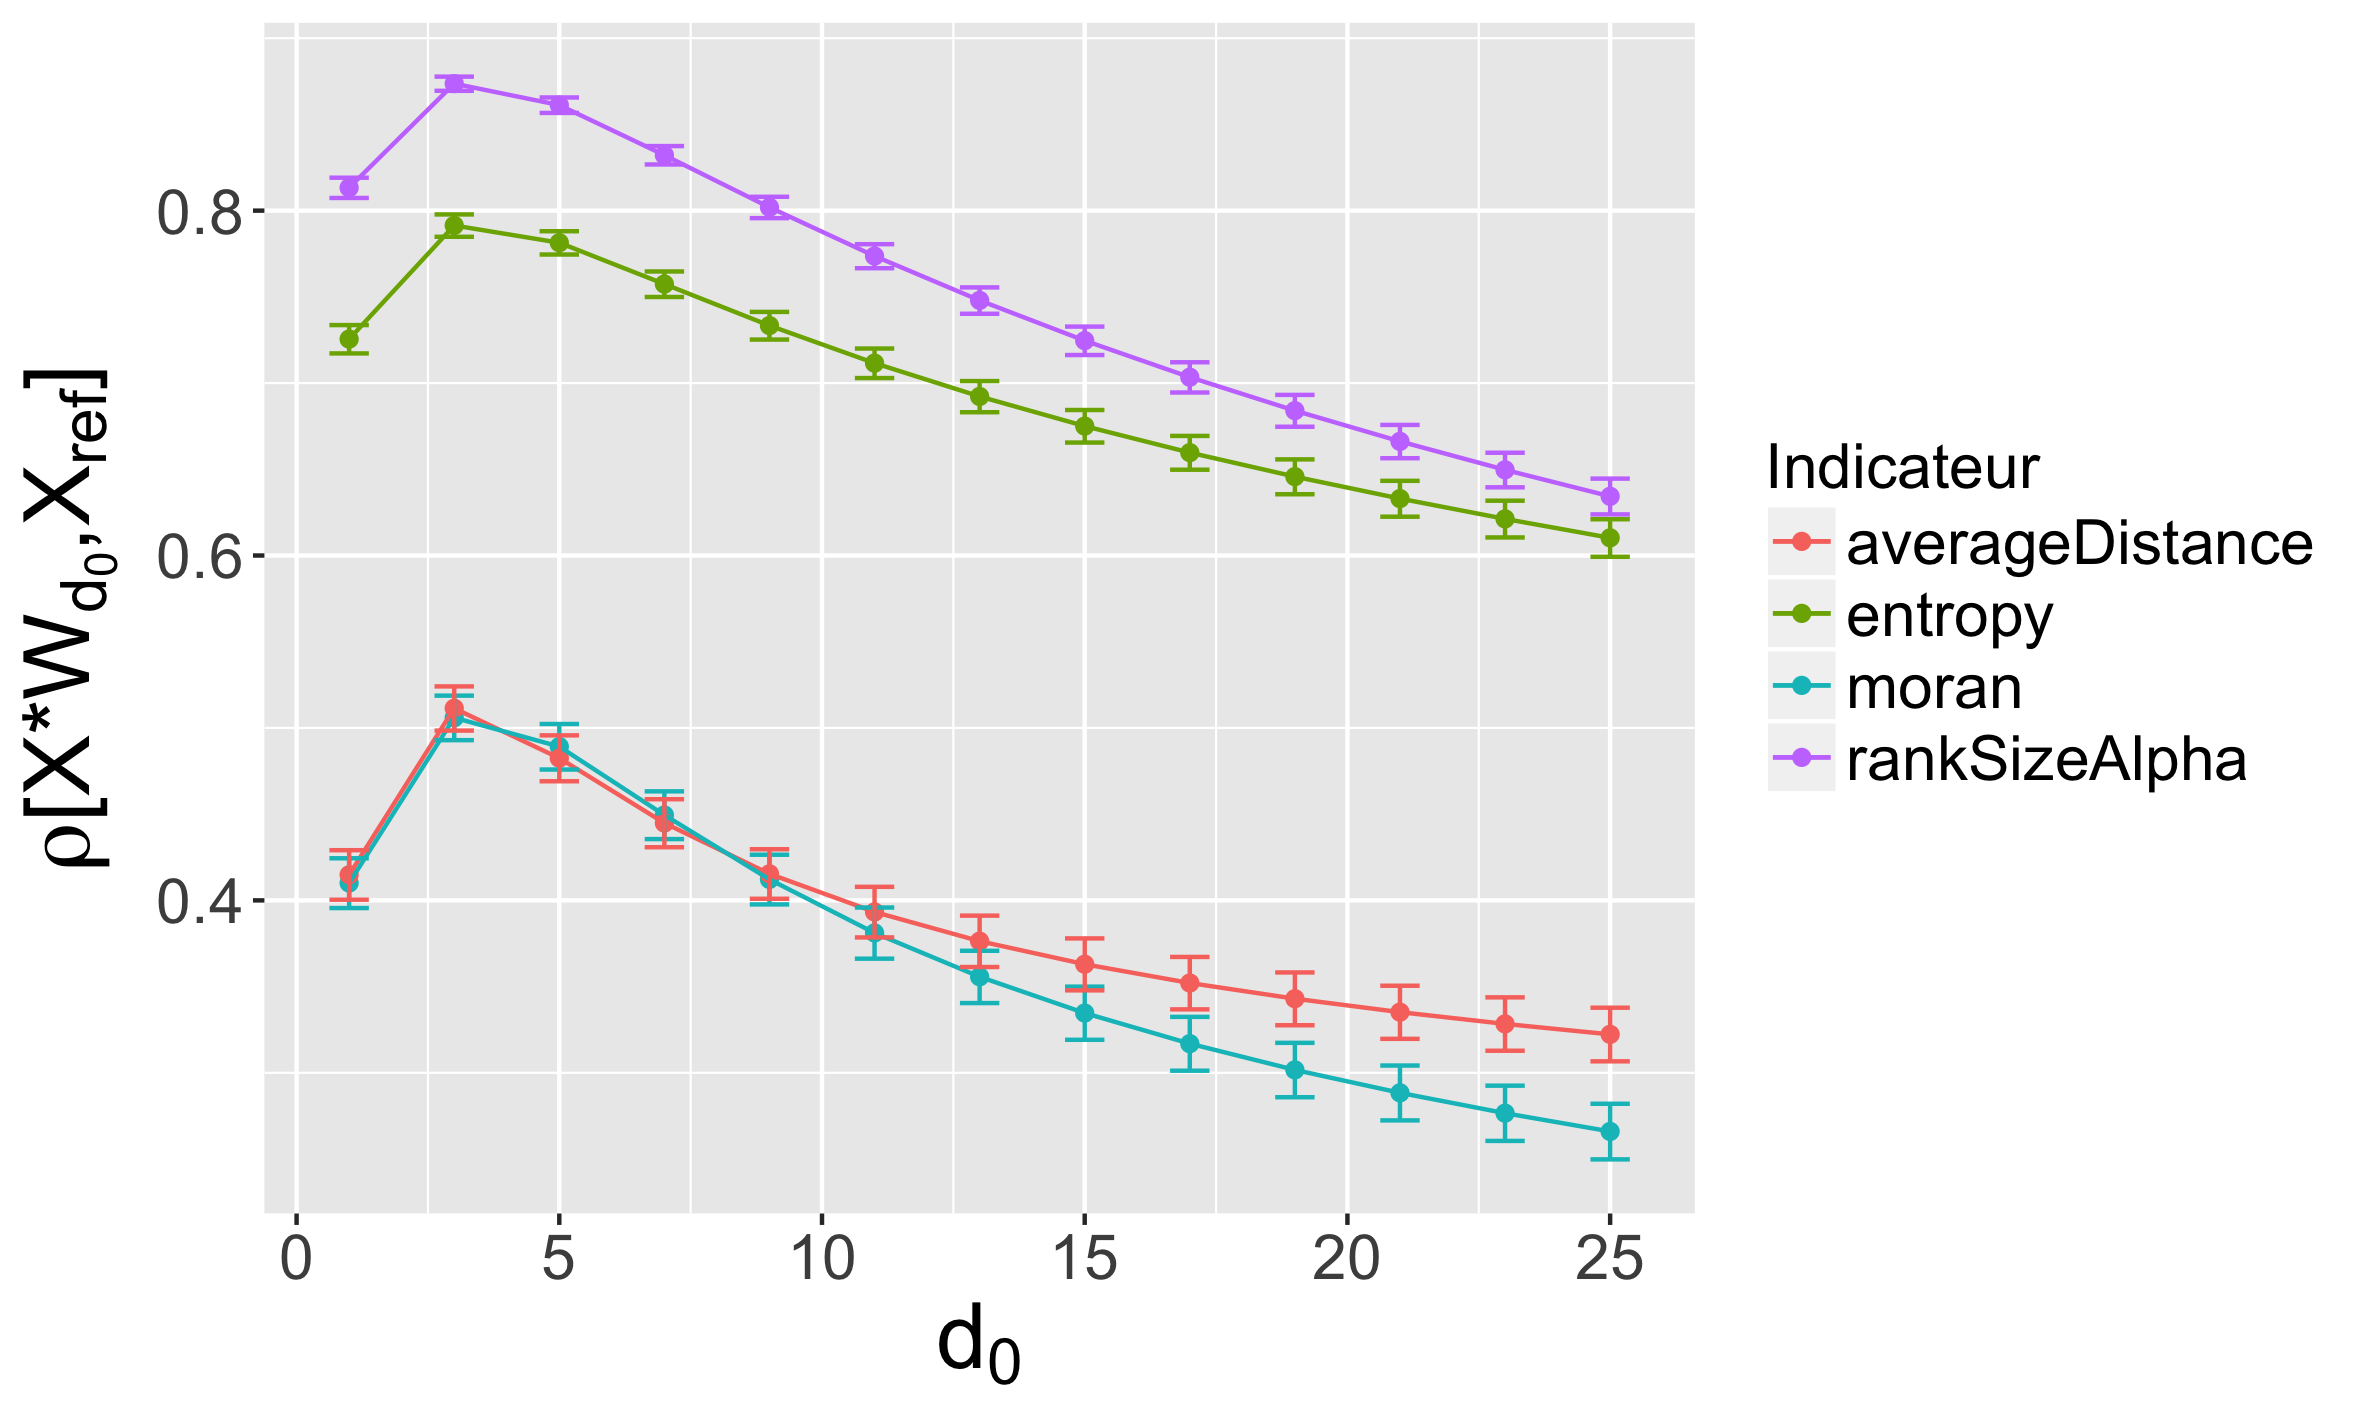
\includegraphics[width=0.48\linewidth]{figuresraw/sensit_morpho_low60_high100.png}
	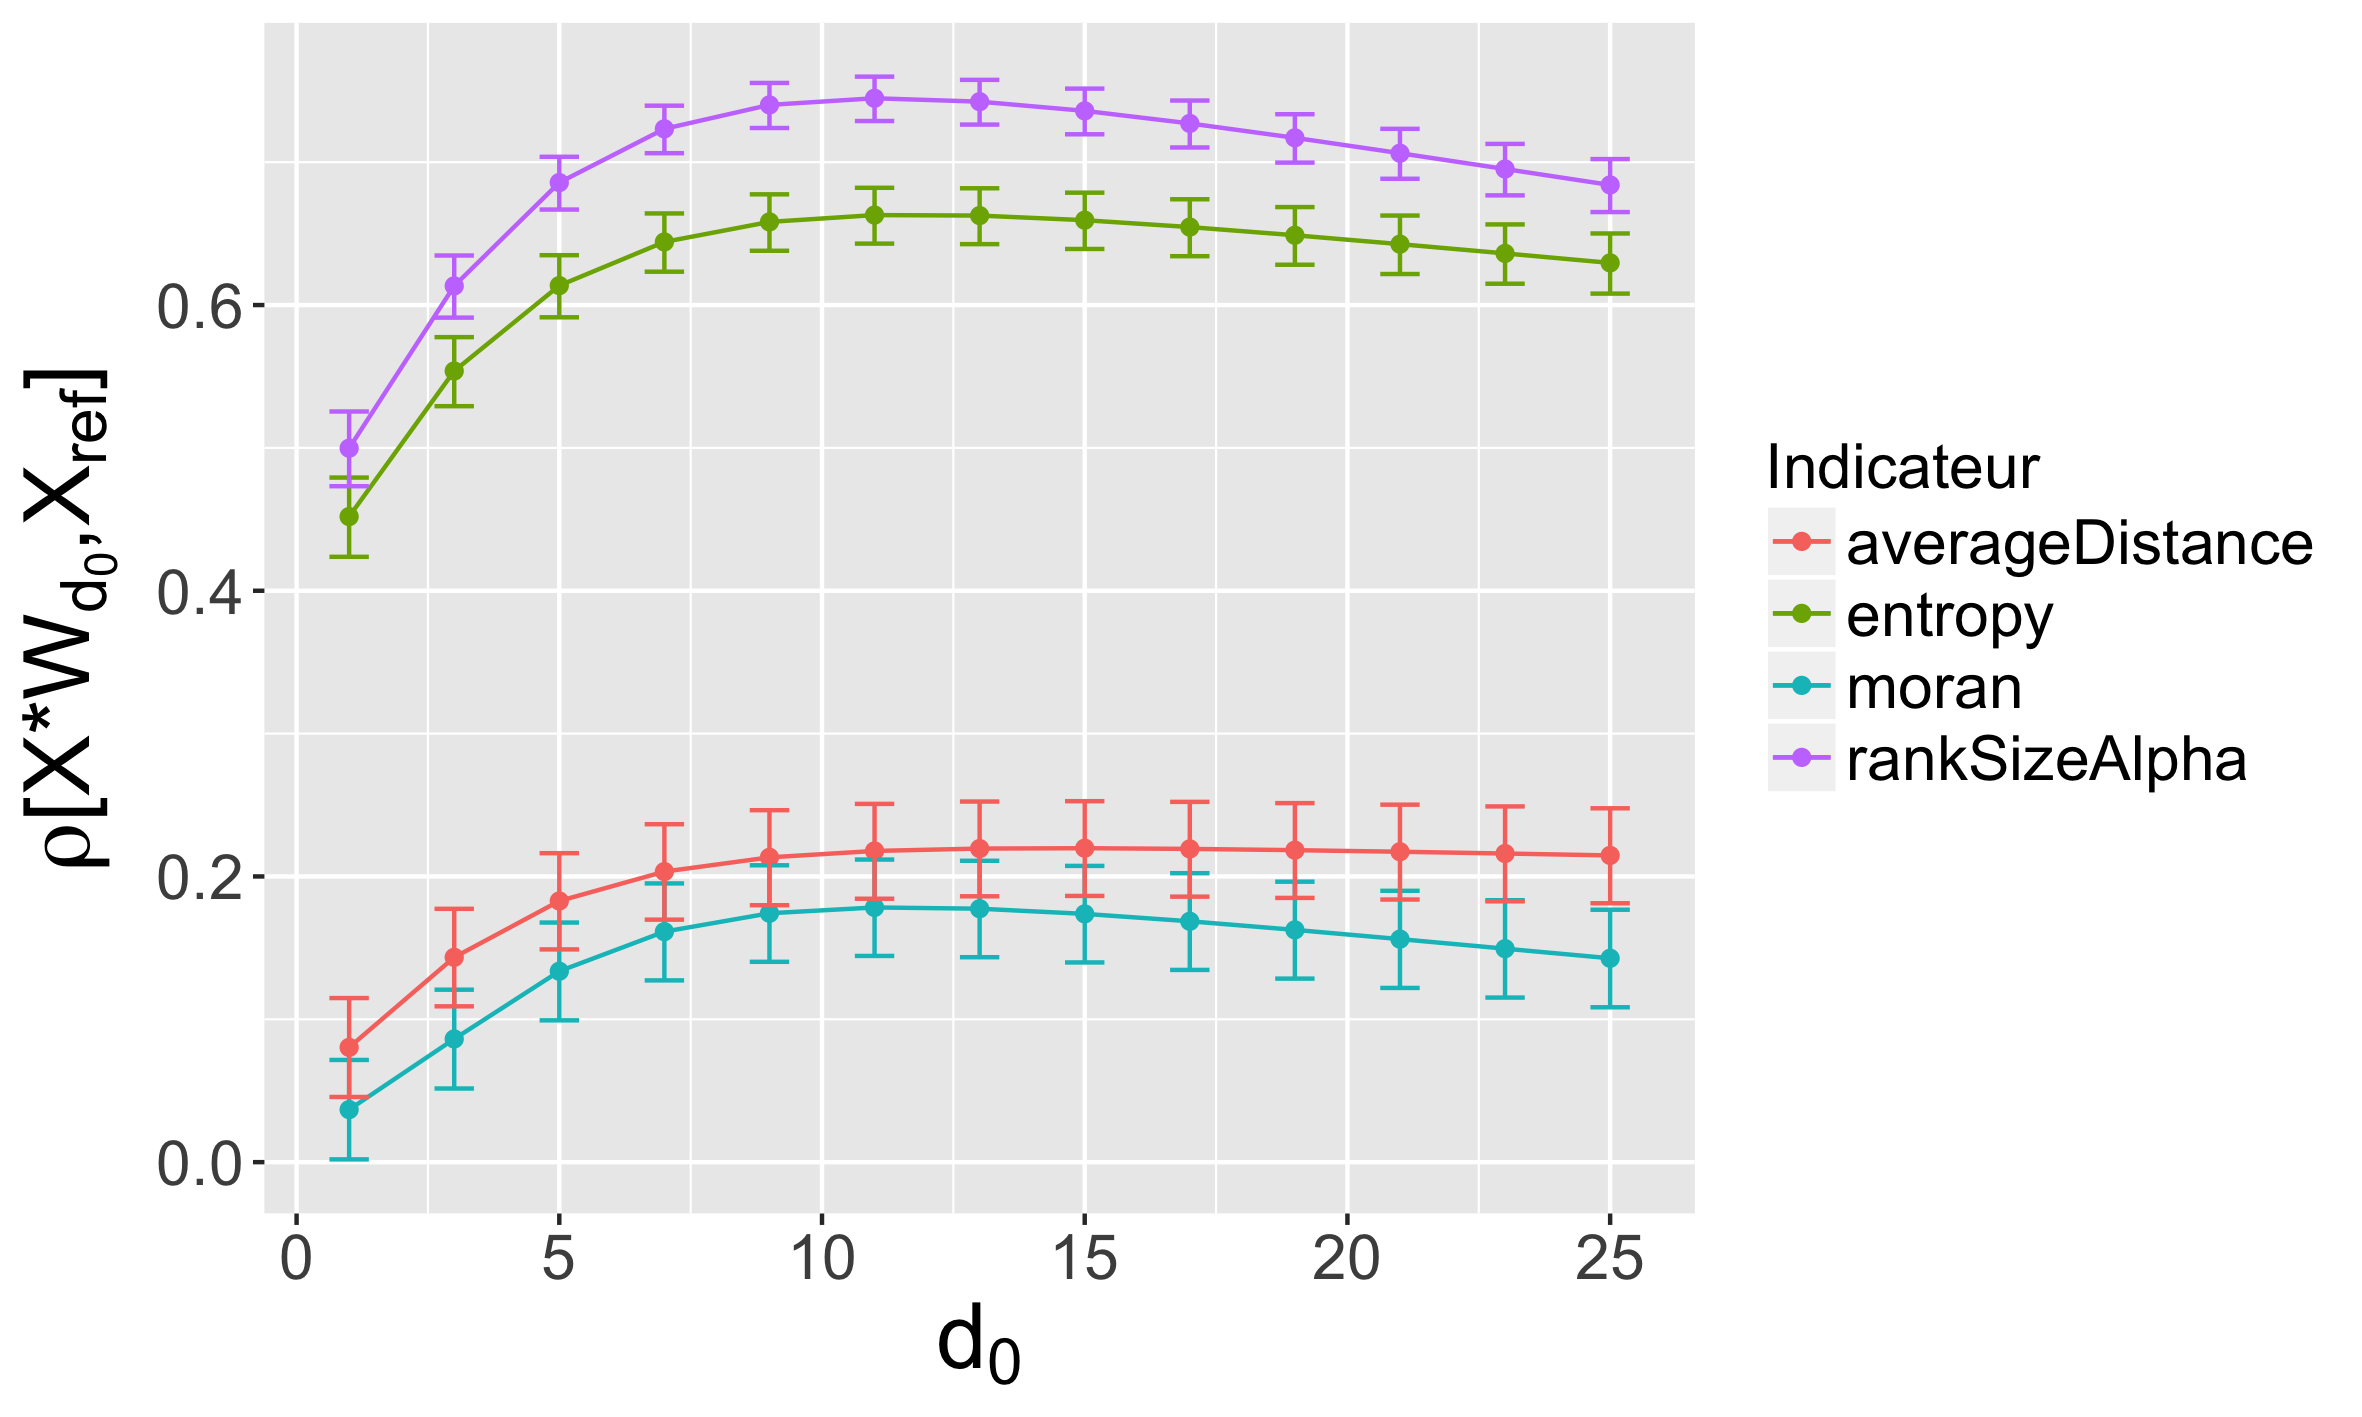
\includegraphics[width=0.48\linewidth]{figuresraw/sensit_morpho_low60_high200.png}\\
	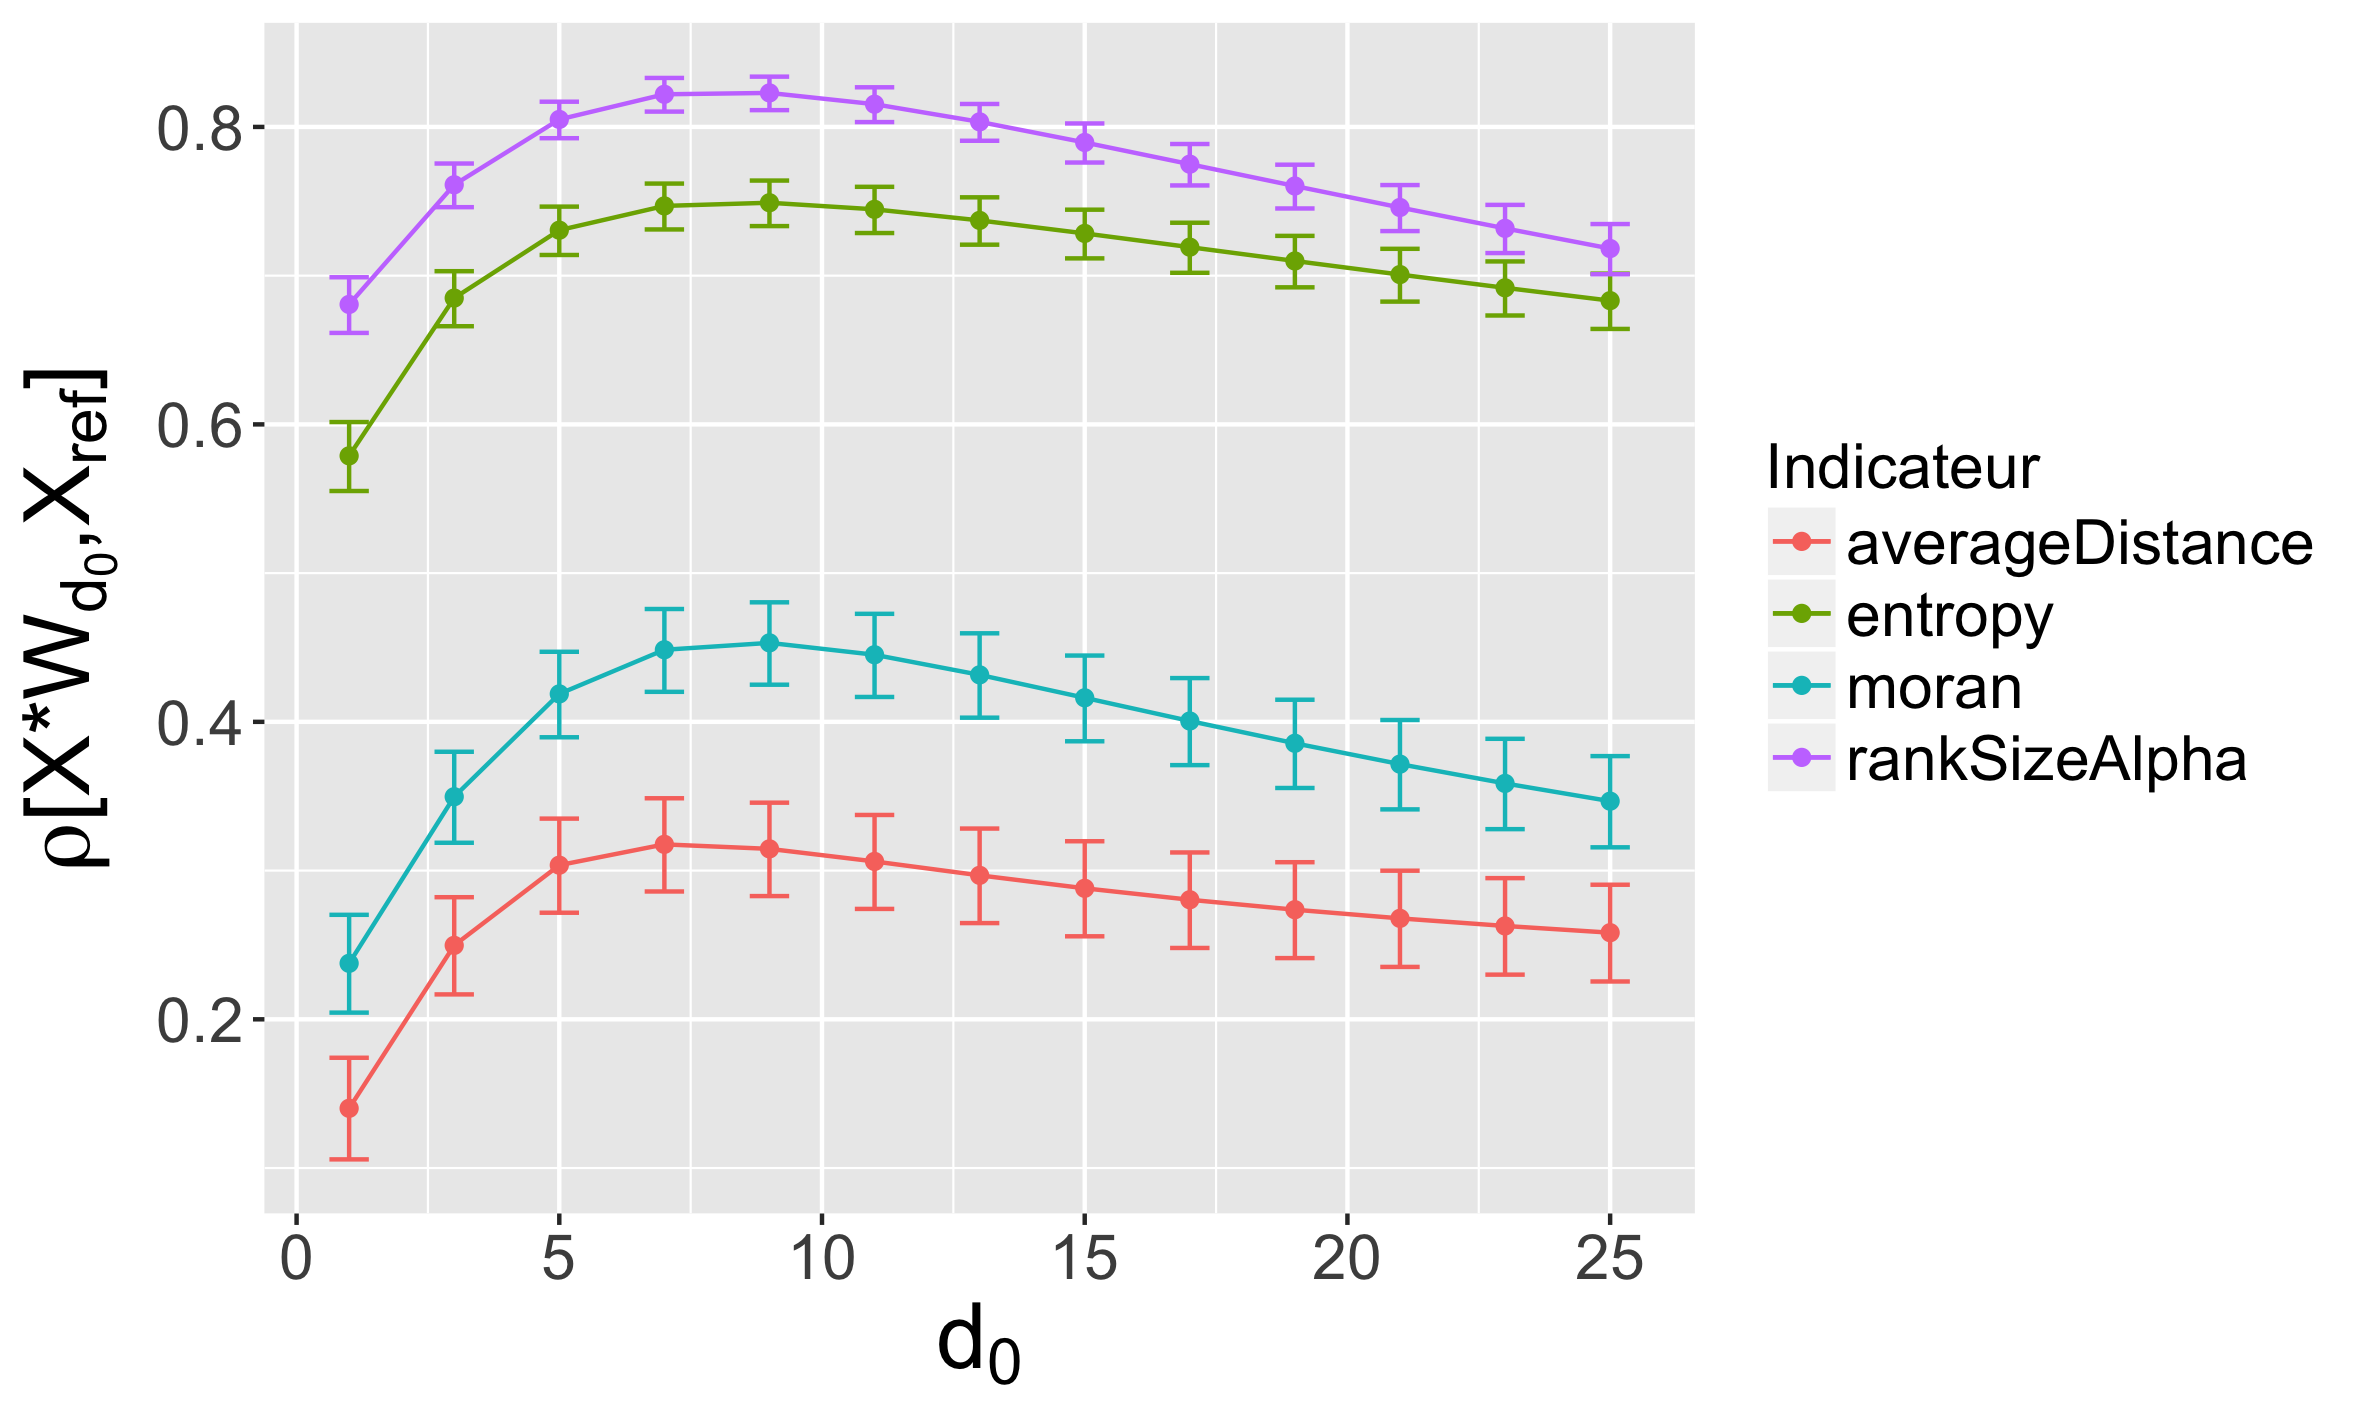
\includegraphics[width=0.48\linewidth]{figuresraw/sensit_morpho_low100_high200.png}
	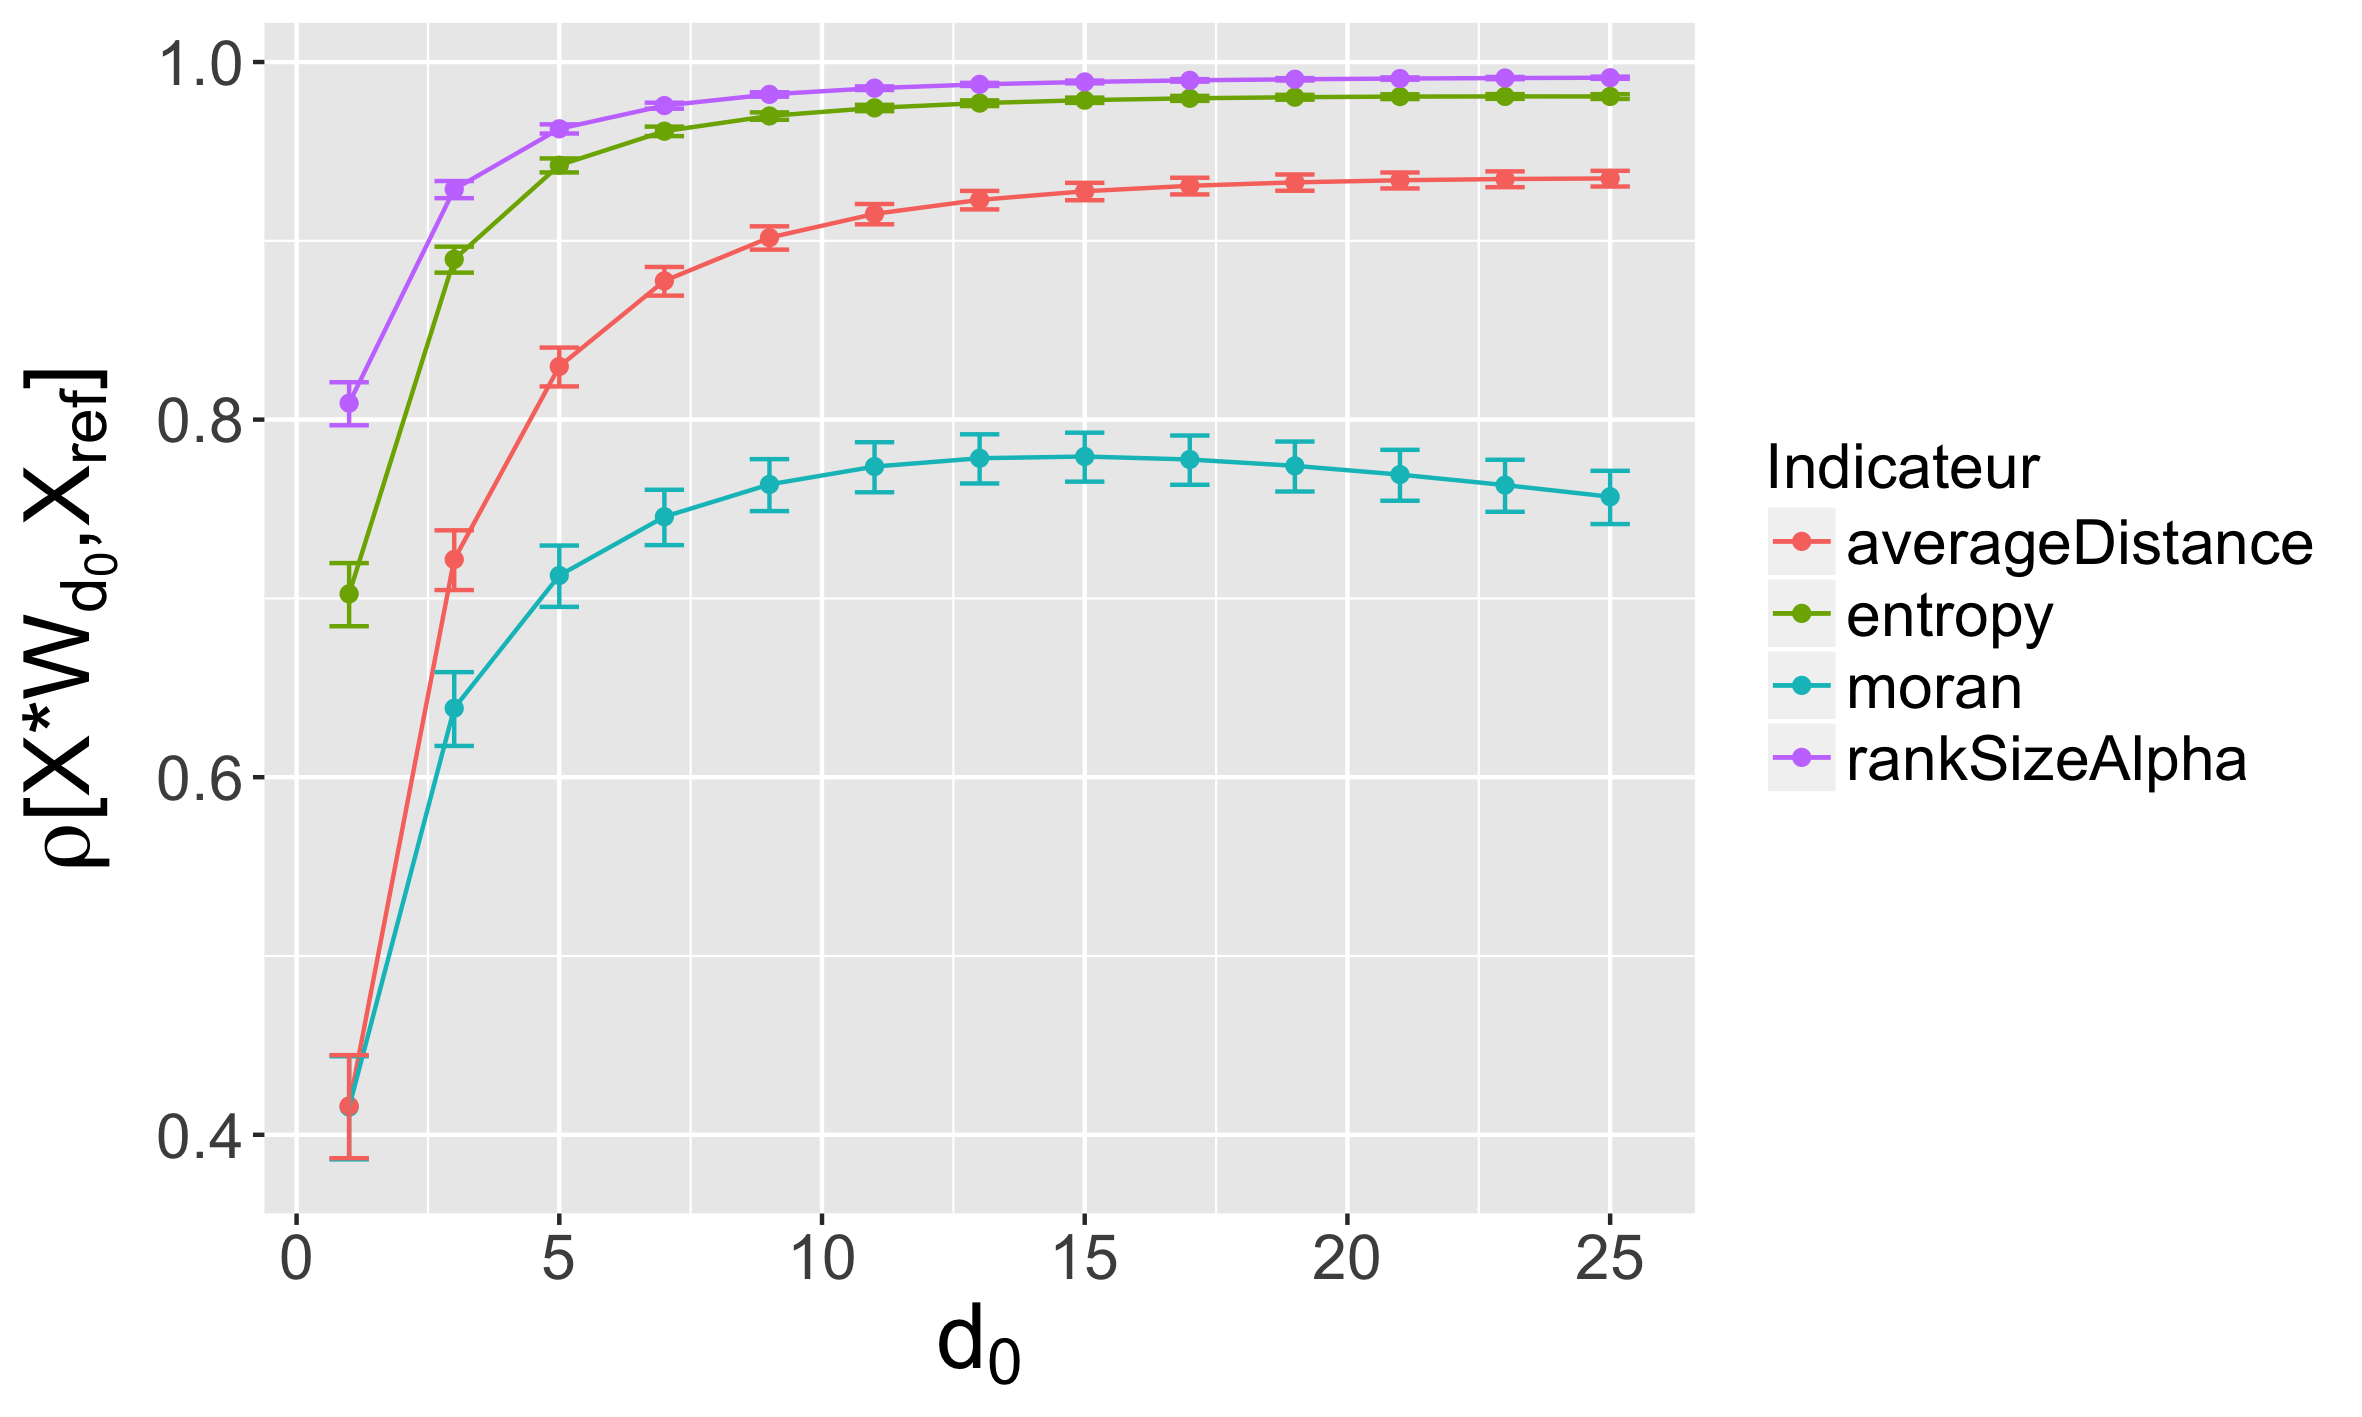
\includegraphics[width=0.48\linewidth]{figuresraw/sensit_morpho_crossed.png}
	\caption{\textbf{Correlations between indicators computed at different scales.} From left to right and top to bottom, $(d=30,D=50)$, $(d=30,D=100)$, $(d=50,D=100)$, and the last plot gives the correlation between the two fields $d_1=30$ and $d_2=50$ both smoothed at the characteristic distance of $d_0$.\label{fig:app:staticcorrelations:sensitivity-corrs}}
\end{figure}
%%%%%%%%%%%%






\end{document}
